\documentclass{bmvc2k}

%% Enter your paper number here for the review copy
%\bmvcreviewcopy{??}

% \usepackage[brazilian]{babel}
\usepackage[utf8]{inputenc}
\usepackage{verbatim}


\title{Projeto Demonstrativo 6\\ Ultilização de uma CNN projetada para classificar imagens no contexto de reconhecimento de fala}

% Enter the paper's authors in order
% \addauthor{Name}{email/homepage}{INSTITUTION_CODE}
\addauthor{Hevelyn Sthefany Lima de Carvalho \\ 170059031}{hevelyn.sthefany@gmail.com}{1}
\addauthor{Igor Bispo de Moraes \\ 170050432}{igor.rabbit99@gmail.com}{1}

% Enter the institutions
% \addinstitution{Name\\Address}
\addinstitution{
  Departamento de Ciência da Comptutação\\
  Universidade de Brasília\\
  Campus Darcy Ribeiro, Asa Norte\\
  Brasília-DF, CEP 70910-900, Brazil,
}

\runninghead{Hevelyn, Igor}{Computer Vision Assignment 5 \today}

% Any macro definitions you would like to include
% These are not defined in the style file, because they don't begin
% with \bmva, so they might conflict with the user's own macros.
% The \bmvaOneDot macro adds a full stop unless there is one in the
% text already.
\def\eg{\emph{e.g}\bmvaOneDot}
\def\Eg{\emph{E.g}\bmvaOneDot}
\def\etal{\emph{et al}\bmvaOneDot}

%-------------------------------------------------------------------------
\begin{document}

\maketitle

\begin{abstract}

O reconhecimento de fala é uma tecnologia que pode reconhecer palavras faladas, que podem ser convertidas em texto. Apresentamos um modelo eficiente para reconhecimento de fala usando a arquitetura MobileNet ~\cite{mobilenets} a qual aplica convoluções separáveis em profundidade. Apresentamos testes obtidos pela rede treinada com forte desempenho e comparamos com os resultados obtidos pela rede com pesos pré-treinados com o ImageNet.

\end{abstract}

%-------------------------------------------------------------------------
\section{Introdução}
\label{sec:intro}

O Reconhecimento de Fala, também conhecido como reconhecimento automático de fala (automatic speech recognition - ASR), reconhecimento de fala por computador ou fala para texto (computer speech recognition or speech to text - STT), é um subcampo de Processamento de Linguagem Natural que se concentra na capacidade e nas limitações de uma máquina em entender a linguagem dos seres humanos. O processo consiste em mapear um entrada de áudio para alguma palavra existente em um certo vocabulário. 

Neste trabalho, transportamos o problema de reconhecimento de áudio para o âmbito de classificação de imagens, uma área muito explorada em Visão Computacional. A análise acústica tem a espectrografia do som como uma de suas principais ferramentas. O espectrograma pode ser definido como uma mostragem dinâmica da densidade de energia por meio do escurecimento ou coloração do traçado (as cores indicam a intensidade de volume), as faixas de frequência no eixo vertical e o tempo no eixo horizontal. Sua representação mostra estrias horizontais, denominadas harmônicos. Um exemplo de espectrograma pode ser vista na Figura ~\ref{espc}. A classificação das imagens foram obtidas através de Rede Neural Convolucional (CNN), mais precisamente, a arquitetura MobileNet ~\cite{mobilenets}.

O conjunto de dados usados para testar, Speech Commands Data Set - versão 0.01, tem um vocabulário relativamente pequeno de 30 ~\cite{speechcommandsv2}. O conjunto compõe-se de falas de 20 palavras de comando gravadas por uma variedade de falantes diferentes:  "Yes", "No", "Up", "Down", "Left", "Right", "On", "Off", "Stop", "Go", "Zero", "One", "Two", "Three", "Four", "Five", "Six", "Seven", "Eight", e "Nine". Para ajudar a distinguir palavras não reconhecidas, há também dez palavras auxiliares:  "Bed", "Bird", "Cat", "Dog", "Happy", "House", "Marvin", "Sheila", "Tree", e "Wow".

Já o conjunto de dados usados para treinar, Speech Commands Data Set - versão 0.02  ~\cite{speechcommandsv2}, inclui as palavras ``backward'', ``follow'', ``forward'', ``learn'' e ``visual''.

Algumas das ferramentas auxiliares principais foram OpenCV ~\cite{openCV} para tratamento de imagens e bibliotecas do Python: Numpy ~\cite{numpy} para manipulação de tensores (imagens), a API Keras para desenvolvimento da rede ~\cite{keras} e o módulo signal do SciPy ~\cite{scipy} para geração dos espectrogramas.


\section{Metodologia}

\subsection*{Pré-processamento}

Para cada audio da base da dados, foram gerados espectrogramas, como visto na figura ~\ref{espc}. O tamanho de cada imagem foi redimensionada para 96x96 afim de diminuir a dimensão do problema. O moedlo de rede usado requer imagem coloridas (RGB), portanto, criamos, para cada imagem, criamos duas novas imagens iguais e as combinamos em uma única imagem de três canais.


\begin{figure}[ht]
\centering
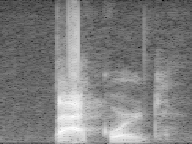
\includegraphics[scale=0.4]{imagens/spect.png} 
\caption{Espectrograma (fala de ``backward'')}
\label{espc}
\end{figure}

\subsection*{Arquitetura da Rede}

MobileNet ~\cite{mobilenets}, proposta pelo Google, foi a arquitetura para a CNN usada neste trabalho a qual usa convoluções separáveis em profundidade.

Uma convolução separável em profundidade é composta por duas operações: uma convolução em profundidade e uma convolução pontual. A convolução em profundidade mapeia uma única convolução em cada canal de entrada separadamente, ou seja, aplica um único filtro a cada canal de entrada (camada  separada para filtragem). Portanto, seu número de canais de saída é o mesmo do número de canais de entrada. Seu custo computacional é $Df^2 \cdot M \cdot Dk^2$, sendo $Df$ a dimensão do recurso de entrada, $M$ e $N$ o número de canais de entrada e saída e $Dk$ o tamanho do kernel. A Figura \ref{MN} (a) e (b)
mostra a diferença entre a Convolução normal e a separável. Já a pontual, Figura \ref{MN} (b) é uma convolução com um tamanho de kernel de 1x1 que combina os recursos criados pela convolução em profundidade (camada separada para combinação), com custo computacional de $M \cdot N \cdot Df^2$.


\begin{figure}[h]
\centering
    \begin{subfigure}[]
        \centering
         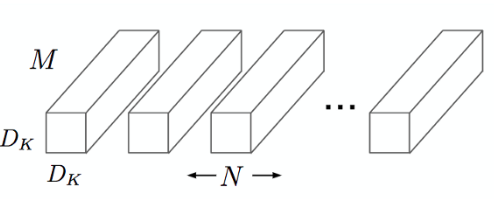
\includegraphics[width=0.4\linewidth]{imagens/mn1.png} 
    \end{subfigure}

    \begin{subfigure}[]
    \centering
         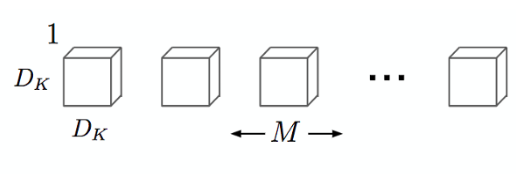
\includegraphics[width=0.4\linewidth]{imagens/mn2.png} ->
         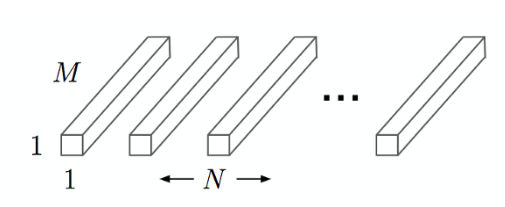
\includegraphics[width=0.4\linewidth]{imagens/mn3.png}
    \end{subfigure}
    \label{MN}
    \caption{Convolução padrão (a) e Convoluções separáveis em Profundidade (b) e (c)~\cite{mobilenets}}
\end{figure}


Todas as camadas são seguidas por uma normalização em lote, batchnorm ~\cite{batch}, especificada na equação abaixo, onde $z^k$ é a camada, $E[x]$ e $V[x]$ são o primeiro e segundo epoch de x respectivamente, e  a função de ativação ReLU ~\cite{relu}, com exceção da camada final totalmente conectada que não possui não-linearidade e alimenta uma camada softmax para classificação.

\begin{equation}
\tilde z ^k = \frac{z^k - E[z^k]}{\sqrt[]{V[z^k]}}
\end{equation}

Os detalhes da arquiterura da rede são mostrados no arquivo Anexo.

\subsection*{Resultados}

\begin{figure}[ht]
\centering
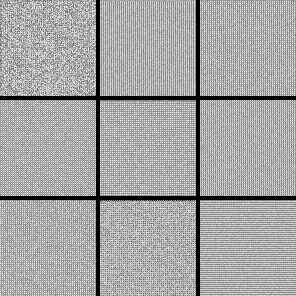
\includegraphics[scale=0.5]{imagens/stitched_filters_3x3.png} 
\caption{Filtros aplicados na Convolução em Profundidade}
\end{figure}

\newpage

\begin{table}[ht]
\centering
\begin{tabular}{|c|c|c|c|c|}
\hline
             & precision  &  recall & f1-score &  support \\ \hline

         bed &      0.95  &    0.98  &    0.97 &      500 \\ \hline
        bird &      0.96  &    0.99  &    0.98 &      500 \\ \hline
         cat &      0.96  &    0.99  &    0.97 &      500 \\ \hline
         dog &      0.97  &    0.96  &    0.97 &      500 \\ \hline
        down &      0.95  &    0.93  &    0.94 &      500 \\ \hline
       eight &      0.95  &    0.97  &    0.96 &      500 \\ \hline
        five &      0.98  &    0.91  &    0.94 &      500 \\ \hline
        four &      0.97  &    0.93  &    0.95 &      500 \\ \hline
          go &      0.88  &    0.95  &    0.92 &      500 \\ \hline
       happy &      1.00  &    0.99  &    0.99 &      500 \\ \hline
       house &      0.99  &    0.99  &    0.99 &      500 \\ \hline
        left &      0.99  &    0.95  &    0.97 &      500 \\ \hline
      marvin &      0.99  &    0.98  &    0.99 &      500 \\ \hline
        nine &      0.96  &    0.95  &    0.96 &      500 \\ \hline
          no &      0.99  &    0.86  &    0.92 &      500 \\ \hline
         off &      0.98  &    0.93  &    0.96 &      500 \\ \hline
          on &      0.95  &    0.94  &    0.95 &      500 \\ \hline
         one &      0.97  &    0.94  &    0.96 &      500 \\ \hline
       right &      0.99  &    0.95  &    0.97 &      500 \\ \hline
       seven &      0.95  &    0.98  &    0.96 &      500 \\ \hline
      sheila &      0.99  &    0.98  &    0.98 &      500 \\ \hline
         six &      0.94  &    0.98  &    0.96 &      500 \\ \hline
        stop &      0.94  &    0.95  &    0.94 &      500 \\ \hline
       three &      0.99  &    0.97  &    0.98 &      500 \\ \hline
         two &      0.97  &    0.96  &    0.96 &      500 \\ \hline
          up &      0.95  &    0.96  &    0.95 &      500 \\ \hline
         wow &      0.98  &    0.98  &    0.98 &      500 \\ \hline
         yes &      0.98  &    0.98  &    0.98 &      500 \\ \hline
        zero &      0.97  &    0.95  &    0.96 &      500 \\ \hline

   micro avg &      0.97   &   0.92  &    0.96 &    14500 \\ 
   macro avg &      0.80   &   0.79  &    0.80 &    14500 \\ 
weighted avg &      0.97   &   0.96  &    0.96 &    14500 \\ \hline
\end{tabular}
\caption{Relatório de Classificação}
\end{table}

\begin{figure}[ht]
\centering
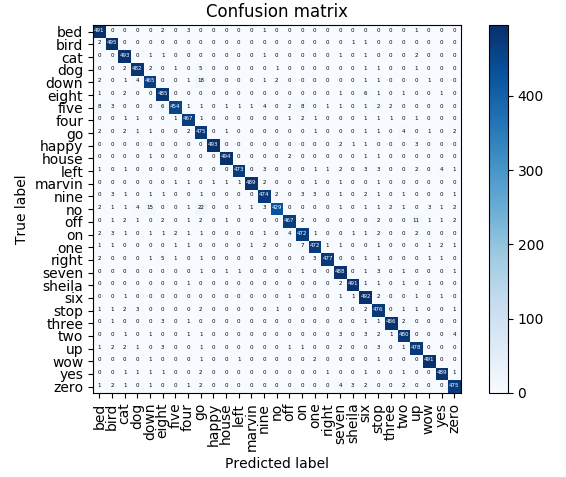
\includegraphics[scale=0.7]{imagens/mtxc.png} 
\caption{Matriz de Confusão - 10 epochs}
\end{figure}

\subsubsection*{Comparação com pesos treinados com ImageNet}

Usamos pesos pré-treinados com o ImageNet ~\cite{imagenet} para comparação. Apesar da base de dados do ImageNet não ter características semelhantes às imagens de espectrograma, pois contém mais de 3 milhões de imagens aleatórias sendo nenhuma espectrograma, o resultado foi indiferente. Além disso, a convergência é mais rápida, atingindo o resultado com 2 epochs a menos que o método anterior.


\section{Conclusão}

Neste projeto foi abordado o problema de reconhecimento de fala aplicando o modelo MobileNet nos dados de imagens formados pelos espectrogramas do banco de dados Speech Commands Data Set. O método foi implementado com sucesso, com 0.97 \% de acurácia.
de precisão. Além disso, destacamos a indiferença entre o método treinando os pesos e o método com os pesos pré treinados com ImageNet, apesar da aleatóriedade deste banco de imagens, no que se trata de acurácia. No entanto, neste segundo método, a convergência é mais rapida.

\newpage
\bibliography{refs}
\end{document}

